\section{Introduction}
%
\label{sec:introduction}

The term tides refers to changes in the shape of an astronomical object in
response to differences in the gravitational pull by a nearby mass at different
locations within the object. In this chapter, tides and their effects are
discussed mostly qualitatively. For a full mathematical description of tides see
\cite{Murray_Dermott_book}.

Consider an exoplanet system consisting of a single planet orbiting a single
star in a circular orbit. The gravitational acceleration due to the star at the
location of the planet's center provides the centripetal acceleration needed to
keep the planet in orbit. The part of the planet facing the star is closer to
the star and therefore experiences a slightly stronger gravitational pull.
However, if we ignore the rotation of the planet for a moment, that part of the
planet must follow a path with the same radius and period as the center of the
planet (though with its center offset slightly). The result is that the star
provides larger gravitational acceleration to that part of the planet than the
required centrifugal acceleration. This excess force is referred to as the tidal
force, and it is directed towards the star for the star-facing part of the
planet. Similarly, on the far side of the planet, the star's gravity is slightly
smaller than what is required to keep that part of the planet in orbit,
resulting in a tidal force pointing away from the star. Relative to the planet
center, both of these forces point outward, causing the planet to elongate along
the star-planet line, and squeeze in the perpendicular direction. This
elongation is frequently referred to as the tidal bulge.

Let us now consider the rotation of the planet. Similarly to tides, rotation
slightly decreases the outward force near the equator of the planet required to
counteract gravity, since part of the gravitational force is required to provide
centripetal acceleration. This causes a slight equatorial bulge. In addition,
rotation interacts with tides. If the period of rotation is exactly equal to the
orbital period (a.k.a. synchronous rotation), the sub-stellar point is fixed on
the planet's surface, and consequently the tidal bulge is also fixed relative to
the planet. However, if the rotation and orbital periods differ, the tidal bulge
will travel on the planet's surface. If the rotational angular velocity of the
planet is $\Omega_{pl}$, and the orbital angular velocity is $\Omega_{orb}$,
the sub-stellar point travel will travel on the surface with an angular
frequency $\Omega_{orb} - \Omega_{pl}$. Since there are two tidal bulges on the
planet (one on the side facing the star and one on the opposite side), the
planetary material will experience a tidal wave with a frequency of
$2(\Omega_{orb} - \Omega_{pl})$.

Any time dependent deformation of the planet will result in some conversion of
mechanical energy to heat. The simplest picture of this is friction between
parts of the planet that move relative to each other. For a continuous medium,
this friction is encapsulated in the concept of viscosity. However, a great
variety of physical processes can result in energy dissipation of tidal
perturbations. The physical causes and the amount of energy that is dissipated
can in principle depend on the internal structure and spin of the planet, as
well as on the frequency and amplitude of the tidal forcing. Regardless of the
causes, this energy dissipation introduces a delay between the tidal forcing and
the response of the planet to that forcing. If the planet spins faster than
synchronous (i.e.  $\Omega_{pl} > \Omega_{orb}$), the tidal bulge will be
carried ahead of the sub-stellar point by the planet's rotation, and if
$\Omega_{pl} < \Omega_{orb}$, the tidal bulge will lag behind
(Fig.~\ref{fig:tidal_bulge}).

\begin{figure}[t]
%
    \centering
%
    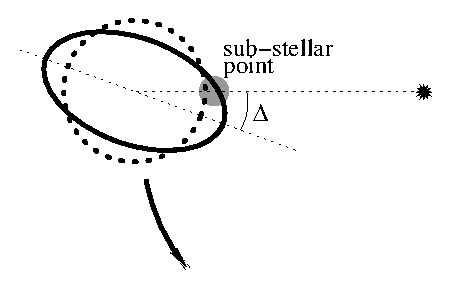
\includegraphics[width=0.5\textwidth]{tidal_bulge.eps}
%
    \caption{
%
        Exaggerated tidal bulge on a planet orbiting a star. Assuming that the
        planet spin angular velocity is smaller than than the orbital angular
        velocity, the tidal bulge will lag behind the sub-stellar point by an
        angle $\Delta$.
%
    }
%
    \label{fig:tidal_bulge}
%
\end{figure}

The two tidal bulges, now shifted relative to the star-planet line, will
experience the gravitational pull of the star. Since the closer bulge will feel
a stronger gravitational force than the farther bulge, there will be a net
torque on the planet. If the bulge is carried ahead of the sub-stellar point by
rotation, the gravitational pull of the star will apply a torque to the planet
opposite to its rotation, acting to slow down its spin, and the reaction force
on the star will act to add angular momentum to the orbit. Conversely, if the
tidal bulge lags behind the sub-stellar point, the gravitational pull of the
star will act to spin the planet up, taking angular momentum out of the orbit.

The discussion above assumed that the equator of the planet is aligned with the
orbital plane. This is not necessarily the case. If the planet's spin is tilted
with respect to the orbit, regardless of whether the planet is rotating faster
or slower than the orbit, rotation will shift the bulges away from the
sub-stellar point in such a way as to produce a torque that will tend over time
to bring the planet's equator and the orbital plane into alignment.

So far we only considered circular orbits. For non-circular orbits, the orbital
angular velocity is no longer constant. It is highest near periapsis (closest
approach between the planet and star) and lowest near apoapsis (largest
planet-star distance). In this case, there exists a spin angular velocity of the
planet, for which the average tidal torque over an orbit vanishes. This is known
as pseudo-synchronous rotation. Near periapsis the orbital angular velocity
exceeds the pseudo-synchronous spin of the planet, thus the tidal bulge leads
the sub-stellar point, causing angular momentum to flow from the orbit to the
planet. Then for the part of the orbit around apoapsis, the orbital angular
velocity is smaller than the pseudo-synchronous spin of the planet, causing
angular momentum to flow in the opposite direction.

\begin{figure}[t]
%
    \centering
%
    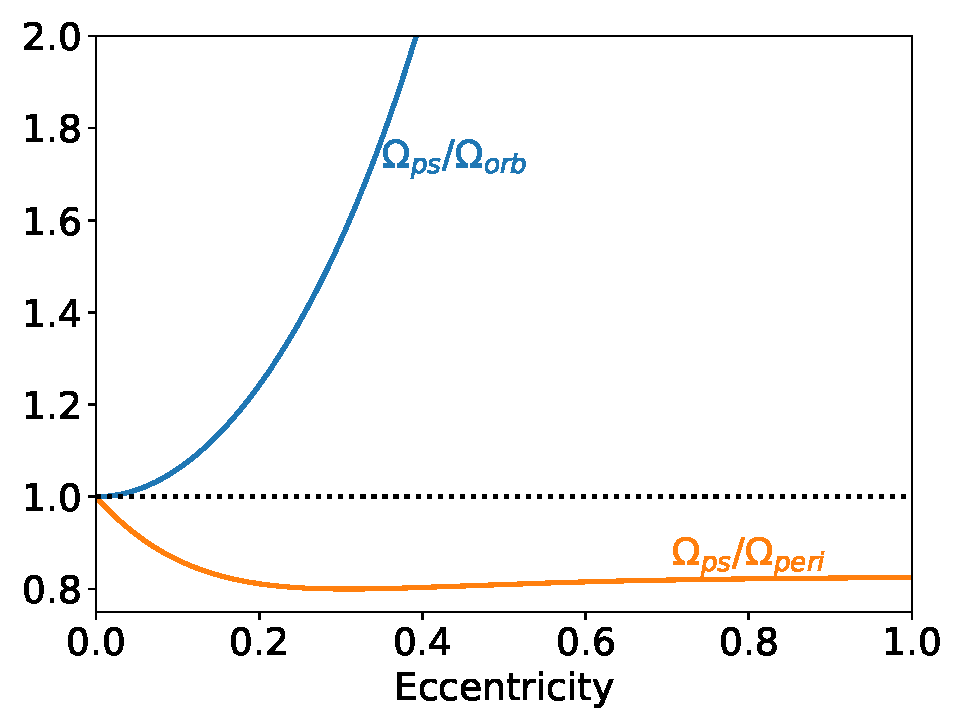
\includegraphics[width=0.5\textwidth]{pseudosync_spin.pdf}
%
    \caption{
%
        The ratio of the pseudo-synchronous spin angular velocity of a planet to
        the average orbital angular velocity and the orbital angular velocity at
        pericenter as a function of the orbital eccentricity assuming the time
        lag of the tidal bulge relative to the tidal forcing is independent of
        the forcing frequency.
%
    }
%
    \label{fig:pseudo-synchronous}
%
\end{figure}


The exact value of the pseudo-synchronous spin depends on the properties of the
tidal dissipation mechanism. \citep{Hut_81} derived an expression for it under
the assumption that all tidal waves experience the same time lag regardless of
the frequency of the tidal forcing giving rise to them. Under that assumption,
since tides are stronger near periapsis, the pseudo-synchronous period must be
somewhat shorter than the orbital period, resulting in the planet being
spun-down over a larger fraction of the orbit than it is being spun up, but at a
slower rate. Thus, the \citet{Hut_81} pseudo-synchronous rotational angular
velocity ($\Omega_{ps}$) of the planet lies between the orbit-average angular
velocity ($\Omega_{orb}$) and the angular velocity at periapsis ($\Omega_{peri}
= \sqrt{(1+e)/(1-e)^3}\Omega_{orb}$). Figure \ref{fig:pseudo-synchronous} shows
the eccentricity dependence of $\Omega_{ps}$ under these assumptions in units of
the orbital angular frequency and the angular frequency at periapsis. If the
spin of the planet is faster(slower) than the pseudo-synchronous rate tides will
act to spin the planet down(up).

For eccentric orbits, even if the planet is pseudo-synchronized, tidal evolution
does not stop. Even though the average torque is zero, energy is still being
dissipated because the sub-stellar point is not fixed on the surface and the
planet-star distance varies over time. From the discussion about
pseudo-synchronous period above, it follows that near periapsis, the sub-stellar
point will drift eastward (i.e. in the direction of rotation), and near apoapsis
it will drift westward, with a long-term westward average, since the
pseudo-synchronous spin period is shorter than the orbital period. These
shifting both in location and amplitude tidal bulges will still experience
energy dissipation. Thus while no angular momentum will be exchanged between the
planet and the orbit, energy will still be extracted from the system and
dissipated as heat, causing the orbit to circularize over time.

Everything we have said so far about the tides the star raises on the planet
applies equally to the tides the planet raises on the star. For circular orbits,
aligned with the stellar equator, if the spin angular velocity of the star
exceeds the orbital angular velocity, angular momentum is transferred from the
stellar spin to the orbit, and if the stellar spin is slower than the orbit,
angular momentum flows in the opposite direction. Similarly, we can define a
pseudo-synchronous period for the star at which the net tidal torque averaged
over a complete orbit vanishes. Even if the star is spinning
pseudo-synchronously, tidal energy dissipation continues and acts to circularize
the orbit over time. For misaligned orbits, tides will gradually work to align
the orbital plane with the stellar equator.

The amplitude of the tidal bulge is set by competition between the tidal force
and the self-gravity of the planet or the star experiencing the tides.
Consequently, the planetary tides are positively correlated with the planet
radius and stellar mass and negatively correlated with the planet mass.
Conversely, the stellar tides are larger for more massive planets and smaller
for larger stellar masses. Both stellar and planetary tides get weaker with
increasing star-planet separation, implying that tides will only be important if
the planet gets close to its parent star for at least some part of its orbit.
This can occur in one of two ways: either the planet has a very small orbital
semimajor axis (short period orbit), or the eccentricity of the planet is very
large making the pericenter distance small.

\section{Tidal timescales}

Based on the discussion above, we can think of four separate tidal evolution
timescales (ordered from shortest to longest):

\begin{enumerate}
%
    \item The timescale on which the planet's spin gets pseudo-synchronized and
        aligned with the orbit
%
    \item The timescale on which the orbit circularizes
%
    \item The timescale on which the orbital period of a circular orbit changes
%
    \item The timescale on which the stellar spin changes
%
\end{enumerate}

All of these timescales are orders of magnitude longer than the orbital period.
If they were not, tides would be strong enough to tear the planet apart. This
allows for a very important simplification when calculating the tidal evolution.
Namely, one can begin by neglecting the evolution of the shape and size of the
orbit, as well as the spins of the two object over a single orbital period.
Under these assumptions, one could calculate the average torque and power due to
tides over an orbital period. The evolution of the orbital elements and stellar
and planetary spins can then be calculated based on these averages.

Let us compare the timescales listed above. We begin by considering the relative
angular momenta of the planet's spin, the orbit, and the stellar spin. The first
scales as the mass of the planet times its radius squared. The second scales as
the mass of the planet times the size of the orbit squared. The third scales as
the mass of the star times the stellar radius squared. Since the planet radius
is tiny compared to the orbit and the planet mass and radius are both very small
compared to the star's, the planet's spin angular momentum is negligible
compared to both the orbital angular momentum and the spin angular momentum of
the star. Consequently, both the direction and period of the planet's spin can
be changed by tides without significantly affecting the orbit, implying that the
timescale on which the planet's spin gets pseudo-synchronized and aligned with
the orbit is negligible compared to the timescales on which the orbit or the
stellar spin evolve. Thus, we can assume that if a given exoplanet orbits close
enough to its star for tides to be important, to a good approximation we can
assume that the planet's spin is aligned with the orbit and pseudo-synchronized.

To compare the two timescales on which the orbit changes (second and third
timescales above), we begin by comparing the importance of the planetary to the
stellar tides. The tidal deformation of an object is set by a competition
between the tidal force due to the companion and the self-gravity of the object
being tidally stretched. Since the planet has a smaller self-gravity and
experiences much larger tidal force than the star, the planet is much more
tidally deformed than the star. Consequently, as long as planetary tides are not
static they will drive faster orbital evolution than the stellar tides. By the
reasoning above, for both circular and eccentric orbits, we expect the planet to
be aligned and spin pseudo-synchronously with the orbit.  Hence, for eccentric
orbits, the planetary tides still contribute to the evolution, while for
circular orbits they do not. This in turn means that the tidal circularization
timescale is shorter than the timescale on which circular orbits change their
period, since the latter is only driven by the much weaker stellar tides.

To compare these timescales to the timescale on which the stellar spin is
affected by tides, note that stars have sufficiently large moment of inertia
for their spin angular momentum to be comparable to or larger than the orbital
angular momentum. Since only the stellar tides can affect the stellar spin, this
implies that the timescale on which the stellar spin changes is comparable to or
longer than the timescale on which the orbital period changes.
